
\documentclass{article} 
\usepackage{iclr2021_conference,times}

\usepackage{hyperref}
\usepackage{url}
\usepackage{lmodern}
\usepackage{amsmath}
\usepackage{amsthm}
\usepackage{amssymb}
\usepackage{amsfonts}
\usepackage{bbm}
\usepackage{graphicx}
\usepackage{subfig}
\usepackage{enumitem}


\def\REF{{\color{red}REF}}

\newcommand\st{~~~\text{s.t.}~~~}
\def\f{\tilde{f}}
\def\eg{\emph{e.g.}}
\def\ie{\emph{i.e.}}
\def\Hcal{{\mathcal H}}
\def\Kcal{{\mathcal K}}
\def\Fcal{{\mathcal F}}
\def\Pcal{{\mathcal P}}
\def\Xcal{{\mathcal X}}
\def\Ycal{{\mathcal Y}}
\def\Ncal{{\mathcal N}}
\def\Real{{\mathbb R}}
\def\vs{}
\def\kmone{{k\text{--}1}}
\def\kmtwo{{k\text{--}2}}
\def\nmone{{n\text{--}1}}
\def\pmone{{p\text{--}1}}
\def\dmone{{d\text{--}1}}
\def\defin{:=}
\def\NTK{{\text{NTK}}}
\def\RF{{\text{RF}}}



\def\x{{\mathbf x}}
\def\L{{\cal L}}
\def\R{{\mathbb R}}
\def\N{{\mathbb N}}
\def\Z{{\mathbb Z}}
\def\Sbb{{\mathbb S}}
\def\Hc{{\mathcal H}}
\def\Hcbar{\bar{\mathcal H}}
\def\activ{\sigma}
\def\sigtot{\sigma_{\text{tot}}}
\def\sigp{\sigma_p}
\def\sigpi{\sigma_i}
\def\sigpq{\sigma_q}

\newcommand*\pFq[2]{{}_{#1}F_{#2}}

\DeclareMathOperator{\Tr}{Tr}
\DeclareMathOperator{\conv}{\textbf{conv}}
\DeclareMathOperator{\dom}{\textbf{dom}}
\DeclareMathOperator{\diag}{diag}
\DeclareMathOperator{\prox}{prox}
\DeclareMathOperator{\vect}{span}
\DeclareMathOperator{\Var}{Var}
\DeclareMathOperator{\cov}{cov}
\DeclareMathOperator{\E}{\mathbb{E}}
\DeclareMathOperator{\1}{\mathbbm{1}}

\newtheorem{theorem}{Theorem}
\newtheorem{proposition}[theorem]{Proposition}
% \newtheorem{remark}[theorem]{Remark}
\newtheorem{lemma}[theorem]{Lemma}
% \newtheorem{definition}[theorem]{Definition}
\newtheorem{corollary}[theorem]{Corollary}
% \newtheorem{example}[theorem]{Example}



\title{Deep Equals Shallow for ReLU Networks \\ in Kernel Regimes}


\author{Alberto Bietti\thanks{Work done while at Inria.} \\
NYU\thanks{Center for Data Science, New York University. New York, USA.} \\
\texttt{alberto.bietti@nyu.edu}
\And
Francis Bach \\
Inria\thanks{Inria - Département d’Informatique de l’École Normale Supérieure.
PSL Research University.
Paris, France.} \\
\texttt{francis.bach@inria.fr} \\
}


\newcommand{\fix}{\marginpar{FIX}}
\newcommand{\new}{\marginpar{NEW}}

\iclrfinalcopy 
\begin{document}


\maketitle

\begin{abstract}
Deep networks are often considered to be more expressive than shallow ones in terms of approximation.
Indeed, certain functions can be approximated by deep networks provably more efficiently than by shallow ones, however, no tractable algorithms are known for learning such deep models.
Separately, a recent line of work has shown that deep networks trained with gradient descent may behave like (tractable) kernel methods in a certain over-parameterized regime, where the kernel is determined by the architecture and initialization, and this paper focuses on approximation for such kernels.
We show that for ReLU activations, the kernels derived from deep fully-connected networks have essentially the same approximation properties as their ``shallow'' two-layer counterpart, namely the same eigenvalue decay for the corresponding integral operator. This highlights the limitations of the kernel framework for understanding the benefits of such deep architectures.
Our main theoretical result relies on characterizing such eigenvalue decays through differentiability properties of the kernel function, which also easily applies to the study of other kernels defined on the~sphere.
\end{abstract}

\section{Introduction}
\label{sec:introduction}
Neural networks currently dominate modern artificial intelligence, however, despite their empirical success establishing a principled theoretical foundation for them remains an active challenge. The key difficulties are that neural networks induce nonconvex optimization objectives \citep{Sontag89backpropagationcan} and typically operate in an overparameterized regime which precludes classical statistical learning theory \citep{DBLP:books/daglib/0025992}. The persistent success of overparameterized models tuned via non-convex optimization suggests that the relationship between the parameterization, optimization, and generalization is more sophisticated than that which can be addressed using classical theory. 
\par
A recent breakthrough on understanding the success of overparameterized networks was established through the Neural Tangent Kernel (NTK) \citep{jacot_ntk}.  In the infinite width limit the optimization dynamics are described entirely by the NTK and the parameterization behaves like a linear model \citep{Lee2019WideNN-SHORT}.  In this regime explicit guarantees for the optimization and generalization can be obtained \citep{du2019gradient,du2018gradient,fine_grain_arora, allenzhu2019convergence, zou2020gradient}.  While one must be judicious when extrapolating insights from the NTK to finite width networks \citep{10.5555/3495724.3496995}, the NTK remains one of the most promising avenues for understanding deep learning on a principled basis.
\par
The spectrum of the NTK is fundamental to both the optimization and generalization of wide networks. In particular, bounding the smallest eigenvalue of the NTK Gram matrix is a staple technique for establishing convergence guarantees for the optimization \citep{du2019gradient,du2018gradient,solt_mod_over}.  Furthermore, the full spectrum of the NTK Gram matrix governs the dynamics of the empirical risk \citep{arora_exact_comp}, and the eigenvalues of the associated integral operator characterize the dynamics of the generalization error outside the training set \citep{bowman2022spectral, bowman2022implicit}. Moreover, the decay rate of the generalization error for Gaussian process regression using the NTK can be characterized by the decay rate of the spectrum \citep{caponnetto2007optimal, cui2021generalization,jin2022learning}. 
\par
The importance of the spectrum of the NTK has led to a variety of efforts to characterize its structure via random matrix theory and other tools \citep{https://doi.org/10.48550/arxiv.1907.10599,NEURIPS2020_572201a4}.  There is a broader body of work studying the closely related Conjugate Kernel, Fisher Information Matrix, and Hessian \citep{Poole2016,pennington_nonlinear,pennington_shallow,10.2307/26542333,Karakida_2020}.  These results often require complex random matrix theory or operate in a regime where the input dimension is sent to infinity.  By contrast, using a just a power series expansion we are able to characterize a variety of attributes of the spectrum for fixed input dimension and recover key results from prior work. 

\subsection{Contributions} 
    In Theorem~\ref{theorem:ntk_power_series} we derive coefficients for the power series expansion of the NTK under unit variance initialization, see Assumption \ref{assumption:init_var_1}. Consequently we are able to derive insights into the NTK spectrum, notably concerning the outlier eigenvalues as well as the asymptotic decay. 
\begin{itemize}[leftmargin=*] 
    \item In Theorem~\ref{thm:infinite_effective_constant_bd} and Observation~\ref{obs:order_one_outliers} we demonstrate that the largest eigenvalue $\lambda_1(\mK)$ of the NTK takes up an $\Omega(1)$ proportion of the trace and that there are $O(1)$ outlier eigenvalues of the same order as $\lambda_1(\mK)$. 
    \item In Theorem~\ref{thm:infinite_effective_rank_bd} and Theorem~\ref{thm:main_effective_rank_bd} we show that the effective rank $Tr(\mK) / \lambda_1(\mK)$ of the NTK is upper bounded by a constant multiple of the effective rank $Tr(\mX \mX^T) / \lambda_1(\mX \mX^T)$ of the input data Gram matrix for both infinite and finite width networks.  
    \item In Corollary~\ref{cor:ReLUbias0} and Theorem~\ref{theorem:informal_ub_eigs_nonuniform} we characterize the asymptotic behavior of the NTK spectrum for both uniform and nonuniform data distributions on the sphere. 
\end{itemize}

\subsection{Related work}
\textbf{Neural Tangent Kernel (NTK):} the NTK was introduced by \cite{jacot_ntk}, who demonstrated that in the infinite width limit neural network optimization is described via a kernel gradient descent.  As a consequence, when the network is polynomially wide in the number of samples, global convergence guarantees for gradient descent can be obtained \citep{du2019gradient,du2018gradient,allenzhu2019convergence, zou2019improved,Lee2019WideNN-SHORT,zou2020gradient,solt_mod_over,marco,nguyenrelu}. Furthermore, the connection between infinite width networks and Gaussian processes, which traces back to \cite{neal1996}, has been reinvigorated in light of the NTK. Recent investigations include  \cite{LeeBNSPS18,matthews2018gaussian,bayesianconv}. 

\textbf{Analysis of NTK Spectrum:} theoretical analysis of the NTK spectrum via random matrix theory was investigated by \cite{https://doi.org/10.48550/arxiv.1907.10599,NEURIPS2020_572201a4} in the high dimensional limit. \cite{NEURIPS2021_14faf969} demonstrated that for ReLU networks the spectrum of the NTK integral operator asymptotically follows a power law, which is consistent with our results for the uniform data distribution. \cite{uniform_sphere_data} calculated the NTK spectrum for shallow ReLU networks under the uniform distribution, which was then expanded to the nonuniform case by \cite{10.5555/3524938.3525002}. \cite{geifman2022on} analyzed the spectrum of the conjugate kernel and NTK for convolutional networks with ReLU activations whose pixels are uniformly distributed on the sphere.  \cite{geifman2020similarity, bietti2021deep,chen2021deep} analyzed the reproducing kernel Hilbert spaces of the NTK for ReLU networks and the Laplace kernel via the decay rate of the spectrum of the kernel.  In contrast to previous works, we are able to address the spectrum in the finite dimensional setting and characterize the impact of different activation functions on it. 

\textbf{Hermite Expansion:} \cite{dual_view} used Hermite expansion to the study the expressivity of the Conjugate Kernel. \cite{pmlr-v162-simon22a} used this technique to demonstrate that any dot product kernel can be realized by the NTK or Conjugate Kernel of a shallow, zero bias network. \cite{solt_mod_over} use Hermite expansion to study the NTK and establish a quantitative bound on the smallest eigenvalue for shallow networks. This approach was incorporated by \cite{marco} to handle convergence for deep networks, with sharp bounds on the smallest NTK eigenvalue for deep ReLU networks provided by \cite{nguyen_tight_bounds}. The Hermite approach was utilized by \cite{Panigrahi2020Effect} to analyze the smallest NTK eigenvalue of shallow networks under various activations. Finally, in a concurrent work \cite{han2022fast} use Hermite expansions to develop a principled and efficient polynomial based approximation algorithm for the NTK and CNTK. In contrast to the aforementioned works, here we employ the Hermite expansion to characterize both the outlier and asymptotic portions of the spectrum for both shallow and deep networks under general activations. 

\section{Preliminaries} \label{subsec:preliminaries}
For our notation, lower case letters, e.g., $x,y$, denote scalars, lower case bold characters, e.g., $\vx, \vy$ are for vectors, and upper case bold characters, e.g., $\mX, \mY$, are for matrices.  For natural numbers $k_1, k_2 \in \mathbb{N}$ we let $[k_1] = \{1, \ldots, k_1\}$ and $[k_2, k_1] = \{k_2, \ldots, k_1\}$. If $k_2>k_1$ then $[k_2,k_1]$ is the empty set. We use $\norm{\cdot}_p$ to denote the $p$-norm of the matrix or vector in question and as default use $\norm{\cdot}$ as the operator or 2-norm respectively. We use $\mathbf{1}_{m \times n} \in \mathbb{R}^{m \times n}$ to denote the matrix with all entries equal to one. We define $\delta_{p=c}$ to take the value $1$ if $p=c$ and be zero otherwise. We will frequently overload scalar functions $\phi:\reals \rightarrow \reals$ by applying them elementwise to vectors and matrices. The entry in the $i$th row and $j$th column of a matrix we access using the notation $[\mX]_{ij}$. The Hadamard or entrywise product of two matrices $\mX, \mY \in \reals^{m \times n}$ we denote $\mX \odot \mY$ as is standard. The $p$th Hadamard power we denote $\mX^{\odot p}$ and define it as the Hadamard product of $\mX$ with itself $p$ times, 
\[
\mX^{\odot p} \defeq \mX \odot \mX \odot \cdots \odot \mX.
\]
Given a Hermitian or symmetric matrix $\mX \in \reals^{n \times n}$, we adopt the convention that $\lambda_i(\mX)$ denotes the $i$th largest eigenvalue,
\[
\lambda_1(\mX) \geq \lambda_2(\mX) \geq \cdots \geq \lambda_n(\mX).
\]
Finally, for a square matrix $\mX \in \mathbb{R}^{n \times n}$ we let $Tr(\mX) = \sum_{i = 1}^n [\mX]_{ii}$ denote the trace.

\subsection{Hermite Expansion}
We say that a function $f\colon \reals \rightarrow \reals$ is square integrable with respect to the standard Gaussian measure $\gamma(z) = \frac{1}{\sqrt{2 \pi}} e^{-z^2/2}$ if $\expec_{X \sim \cN(0,1)}[f(X)^2]< \infty$. 
We denote by $L^2(\reals,\gamma)$ the space of all such functions. The normalized probabilist's Hermite polynomials are defined as
\begin{align*}
	h_k(x)=\frac{{(-1)}^ke^{x^2/2}}{\sqrt{k!}} \frac{d^{k}}{d x^{k}} e^{-x^2/2}, \quad k=0,1,\ldots 
\end{align*}
and form a complete orthonormal basis in $L^2(\reals,\gamma)$ \cite[\S 11]{donnellbook}. The Hermite expansion of a function $\phi \in L^2(\reals ,\gamma)$ is given by $\phi(x)= \sum_{k=0}^\infty \mu_k(\phi) h_k(x)$, where $\mu_k(\phi) = \expec_{X \sim \cN(0,1)}[\phi(X)h_k(X)]$ is the $k$th normalized probabilist's Hermite coefficient of $\phi$. 

\subsection{NTK Parametrization} 
In what follows, for $n,d\in \naturals$ let $\mX \in \reals^{n \times d}$ denote a matrix which stores $n$ points in $\reals^d$ row-wise. Unless otherwise stated, we assume $d \leq n$ and denote the $i$th row of $\mX_n$ as $\vx_i$. In this work we consider fully-connected neural networks of the form $f^{(L+1)}\colon \reals^d \rightarrow \reals$ with $L \in \naturals$ hidden layers and a linear output layer. For a given input vector $\vx \in \reals^d$, the activation $f^{(l)}$ and preactivation $g^{(l)}$ at each layer $l \in [L+1]$ are defined via the following recurrence relations, 
\begin{equation}\label{eq:ffnn}
    \begin{aligned}
    &g^{(1)}(\vx) = \gamma_w \mW^{(1)}\vx + \gamma_b\vb^{(1)}, \; f^{(1)}(\vx) = \phi \left( g^{(1)} (\vx) \right),\\
    &g^{(l)}(\vx) = \frac{\sigma_w}{\sqrt{m_{l-1}}} \mW^{(l)} f^{(l-1)}(\vx) + \sigma_b\vb^{(l)}, \; f^{(l)}(\vx) = \phi \left( g^{(l)} (\vx) \right), \; \forall l \in [2,L],\\
    &g^{(L+1)}(\vx) =  \frac{\sigma_w}{\sqrt{m_L}}\mW^{(L+1)}f^{(L)}(\vx), \; f^{(L+1)}(\vx) = g^{(L+1)}(\vx). 
    \end{aligned}
\end{equation}
The parameters $\mW^{(l)} \in \reals^{m_l \times m_{l-1}}$ and $\vb^{(l)} \in \reals^{m_l}$ are the weight matrix and bias vector at the $l$th layer respectively, $m_0 = d$, $m_{L+1} = 1$, and $\phi\colon \reals \rightarrow \reals$ is the activation function applied elementwise. The variables $\gamma_w, \sigma_w \in \reals_{>0}$ and $\gamma_b, \sigma_b \in \reals_{\geq0}$ correspond to weight and bias hyperparameters respectively.
Let $\theta_l \in \reals^p$ denote a vector storing the network parameters $(\mW^{(h)}, \vb^{(h)})_{h=1}^{l}$ up to and including the $l$th layer. The Neural Tangent Kernel \citep{jacot_ntk} $\tilde{\Theta}^{(l)}\colon \reals^d \times \reals^d \rightarrow \reals$ associated with $f^{(l)}$ at layer $l \in [L+1]$ is defined as
\begin{equation} \label{eq:ntk}
    \tilde{\Theta}^{(l)}(\vx, \vy) := \langle \nabla_{\theta_l} f^{(l)}(\vx), \nabla_{\theta_l} f^{(l)}(\vy) \rangle. 
\end{equation}
We will mostly study the NTK under the following standard assumptions.
\begin{assumption}\label{assumptions:kernel_regime}
NTK initialization. 
    \begin{enumerate}[leftmargin=*]
        \item At initialization all network parameters are distributed as $\cN(0,1)$ and are mutually independent.
        \item The activation function satisfies $\phi \in L^2(\reals, \gamma)$, is differentiable almost everywhere and its derivative, which we denote $\phi'$, also satisfies $\phi' \in L^2(\reals, \gamma)$.
        \item The widths are sent to infinity in sequence, $m_1 \rightarrow \infty, m_2 \rightarrow \infty, \ldots, m_{L}\rightarrow \infty$. %We refer to this regime as the sequential infinite width limit. 
    \end{enumerate}
\end{assumption}
Under Assumption~\ref{assumptions:kernel_regime}, for any $l \in [L+1]$, $\tilde{\Theta}^{(l)}(\vx, \vy)$ converges in probability to a deterministic limit $\Theta^{(l)}\colon \reals^d \times \reals^d \rightarrow \reals$ \citep{jacot_ntk} and the network behaves like a kernelized linear predictor during training; see, e.g., \cite{arora_exact_comp, Lee2019WideNN-SHORT, pmlr-v125-woodworth20a}. Given access to the rows $(\vx_i)_{i=1}^n$ of $\mX$ the NTK matrix at layer $l\in [L+1]$, which we denote $\mK_{l}$, is the $n \times n$ matrix with entries defined as 
\begin{equation} \label{eq:ntk_matrix_def}
[\mK_{l}]_{ij} = \frac{1}{n}\Theta^{(l)}(\vx_i, \vx_j), \; \forall (i,j) \in [n] \times [n].
\end{equation}



\section{Review of Approximation with Dot-Product Kernels}
\label{sec:background}

\section{Background}\label{sec:Background}

In the present paper, we derive bounds on the Lipschitz constant of random ReLU networks at initialization.
We consider a variant of the so-called \emph{He initialization} as introduced in \cite{he2015delving}.
In \cite{he2015delving}, the entries of the weight matrices $W^{(\ell)} \in \RR^{N^{(\ell + 1)} \times N^{(\ell)}}$ are identically and independently drawn from a Gaussian distribution
with zero mean and standard deviation $\sqrt{2/N^{(\ell)}}$
and the biases are initialized to zero.
We consider a standard deviation of $\sqrt{2/N^{(\ell+1)}}$, which is commonly used in theoretical studies of random ReLU networks (cf. \cite{buchanan2021deep,allen2019convergence,dirksen2022separation}).
This random initialization is a natural choice since it is \emph{isometric in expectation}, 
meaning that $\EE [\Vert \relu(W^{(\ell)}x)\Vert_2^2] = \Vert x \Vert_2^2$ 
for every vector $x \in \RR^{N^{(\ell)}}$ that is fed into the $\ell$th layer of the network.
Since the $\relu$ is positively homogeneous, our results readily imply corresponding bounds for other initialization choices where the network weights are chosen from a Gaussian distribution which may vary from layer to layer.

Moreover, we allow more general biases than in \cite{he2015delving}.
Specifically, we require that the biases are also drawn independently from certain probability distributions.
In order to derive upper bounds for the Lipschitz constant (see \Cref{sec:upper}) 
and lower bounds in the case of shallow networks (see \Cref{sec:low_bound_shallow}),
we do not need to impose \emph{any} assumptions on these probability distributions.
To derive lower bounds in the case of deep networks (see \Cref{subsec:deep_lower}), however,
we require these probability distributions to be symmetric.
Note that assuming symmetry of the distributions of the biases is very natural and in particular covers
the zero initialization that is used in \cite{he2015delving}.
In the following assumption, we formally introduce the considered random initialization.

\begin{assumption} \label{assum:1}
We consider ReLU networks with $d$ input neurons, 1 output neuron, a width of $N$ and $L$ hidden layers.
Precisely, we consider maps 
\begin{equation} \label{eq:relu-network}
  \Phi: \quad \RR^d \to \RR,
  \quad
  \Phi(x)
  \defeq \left( V^{(L)} \circ \relu \circ V^{(L-1)} \circ  \hdots \circ \relu \circ V^{(0)}\right) (x).
\end{equation}
Here, $\relu$ denotes the function defined as 
\begin{equation*}
  \relu (x) \defeq \max \{0,x\}, \quad x \in \RR,
\end{equation*} 
and the application of $\relu$ in \eqref{eq:relu-network} is to be understood componentwise, i.e., 
\begin{equation*}
  \relu ((x_1, ..., x_N)) = (\relu (x_1),..., \relu(x_N)). 
\end{equation*}
Furthermore, the maps $V^{(\ell)}$ for $0 \leq \ell \leq L$ are affine-linear maps,
which in detail means the following:
There are matrices $W^{(0)} \in \RR^{N \times d}$, $W^{(\ell)} \in \RR^{N \times N}$
for $1 \leq \ell \leq L-1$ and $W^{(L)} \in \RR^{1 \times N}$
as well as \emph{biases} $b^{(\ell)} \in \RR^N$ for $0 \leq \ell < L$ and $b^{(L)} \in \RR$ such that
\begin{equation*}
  V^{(\ell)} (x) = W^{(\ell)}x + b^{(\ell)}
  \quad \text{for every } 0 \leq \ell \leq L.
\end{equation*}

We assume that the matrices $W^{(\ell)}$ as well as the biases $b^{(\ell)}$ are randomly
chosen in the following way:
For $0 \leq \ell < L$, we have 
\begin{equation*}
  \left( W^{(\ell)}\right)_{i,j} \overset{\mathrm{i.i.d.}}{\sim} \mathcal{N}(0,2/N),
  \quad
  \left( W^{(L)}\right)_{1,j} \overset{\mathrm{i.i.d.}}{\sim} \mathcal{N}(0,1).
\end{equation*}
Concerning the biases, we assume
\begin{equation*}
  \left( b^{(\ell)}\right)_i \sim \mathcal{D}^{(\ell)}_i,
  \quad 0 \leq \ell \leq L.
\end{equation*}
Here, each $\mathcal{D}^{(\ell)}_i$ is an arbitrary probability distribution over $\RR$.
Furthermore, the random variables $W^{(0)}, ..., W^{(L)}, b^{(0)}, ..., b^{(L)}$ are assumed to be jointly independent.
\end{assumption}

The above assumption, which suffices for deriving the upper bound on the Lipschitz constant for networks of arbitrary depth and the lower bound in the case of shallow networks,
imposes almost no restrictions on the distribution of the biases.
However, for deriving lower bounds \paul{for deep networks} we will use the following more restrictive assumption
on the initialization of the biases.
\begin{assumption}\label{assum:2}
  Let $\Phi: \RR^d \to \RR$ be a random ReLU network satisfying \Cref{assum:1}.
  Moreover, we assume that each $\mathcal{D}_i^{(\ell)}$ is a symmetric probability distribution over $\RR$
  (e.g., $\mathcal{N}(0, \sigma^2)$ for some parameter $\sigma > 0$, uniform on some interval $[-m,m] \subseteq \RR$, or initialized to zero).
\end{assumption}

We restrict ourselves to square matrices
(i.e., we assume that each layer of the network has the same amount of neurons).
We believe, however, that our proofs still work in the case of layers with varying widths
that are uniformly bounded from below by $\Omega (dL^2)$.



\section{Main Result and Applications to Deep Networks}
\label{sec:approx}


In this section, we present our main results concerning approximation properties of dot-product kernels on the sphere, and applications to the kernels arising from wide random neural networks.
We begin by stating our main theorem, which provides eigenvalue decays for dot-product kernels from differentiability properties of the kernel function~$\kappa$ at the endpoints~$\pm 1$.
We then present applications of this result to various kernels, including those coming from deep networks, showing in particular that the RKHSs associated to deep and shallow ReLU networks are the same (up to parity constraints).

\subsection{Statement of our main theorem}

We now state our main result regarding the asymptotic eigenvalue decay of dot-product kernels.
Recall that we consider a kernel of the form~$k(x, y) = \kappa(x^\top y)$ for~$x, y \in \Sbb^{\dmone}$,
and seek to obtain decay estimates on the eigenvalues~$\mu_k$ defined in~\eqref{eq:mu_k}.
We now state our main theorem, which derives the asymptotic decay of~$\mu_k$ with~$k$ in terms of differentiability properties of~$\kappa$ around~$\{\pm 1\}$, assuming that~$\kappa$ is infinitely differentiable on~$(-1,1)$. This latter condition is always verified when~$\kappa$ takes the form of a power series~\eqref{eq:kappa_series} with~$\kappa(1) = 1$, since the radius of convergence is at least~$1$.
We also require a technical condition, namely the ability to ``differentiate asymptotic expansions'' of~$\kappa$ at~$\pm 1$, which holds for the kernels considered in this work.

\begin{theorem}[Decay from regularity of~$\kappa$ at endpoints, simplified]
\label{thm:decay}
Let~$\kappa: [-1,1] \to \R$ be a function that is~$C^\infty$ on~$(-1,1)$ and has the following asymptotic expansions around~$\pm 1$:
\begin{align}
\kappa(1-t) &= p_1(t) + c_{1} t^{\nu} + o(t^{\nu}) \\
\kappa(-1+t) &= p_{-1}(t) + c_{-1} t^{\nu} + o(t^{\nu}),
\end{align}
for~$t \geq 0$, where~$p_1, p_{-1}$ are polynomials and~$\nu > 0$ is not an integer.
Also, assume that the derivatives of~$\kappa$ admit similar expansions obtained by differentiating the above ones.
Then, there is an absolute constant~$C(d,\nu)$ depending on~$d$ and~$\nu$ such that:
\begin{itemize}[noitemsep]
	\item For~$k$ even, if~$c_1 \ne -c_{-1}$: $\mu_k \sim (c_1 + c_{-1}) C(d,\nu) k^{-d-2 \nu + 1}$;
	\item For~$k$ odd, if~$c_1 \ne c_{-1}$: $\mu_k \sim (c_1 - c_{-1}) C(d,\nu) k^{-d-2 \nu + 1}$.
\end{itemize}
In the case~$|c_1| = |c_{-1}|$, then we have~$\mu_k = o(k^{-d-2 \nu + 1})$ for one of the two parities (or both if~$c_1 = c_{-1} = 0$).
If~$\kappa$ is infinitely differentiable on~$[-1, 1]$ so that no such~$\nu$ exists, then~$\mu_k$ decays faster than any polynomial.
\end{theorem}

The full theorem is given in Appendix~\ref{sec:appx_thm_proof} along with its proof, and requires an additional mild technical condition on the expansion which is verified for all kernels considered in this paper, namely, a finite number of terms in the expansions with exponents between~$\nu$ and~$\nu+1$.
The proof relies on integration by parts using properties of Legendre polynomials, in a way reminiscent of fast decays of Fourier series for differentiable functions, and on precise computations of the decay for simple functions of the form~$t \mapsto (1 - t^2)^\nu$.
This allows us to obtain the asymptotic decay for general kernel functions~$\kappa$ as long as the behavior around the endpoints is known, in contrast to previous approaches which rely on the precise form of~$\kappa$, or of the corresponding activation in the case of arc-cosine kernels~\citep{bach2017breaking,basri2019convergence,bietti2019inductive,geifman2020similarity}.
This enables the study of more general and complex kernels, such as those arising from deep networks, as discussed below.
When~$\kappa$ is of the form~$\kappa(t) = \sum_k b_k t^k$, the exponent~$\nu$ in Theorem~\ref{thm:decay} is also related to the decay of coefficients~$b_k$.
Such coefficients provide a dimension-free description of the kernel which may be useful for instance in the study of kernel methods in certain high-dimensional regimes~\citep[see, \eg,][]{el2010spectrum,ghorbani2019linearized,liang2019risk}.
We show in Appendix~\ref{sub:appx_dimension_free} that the~$b_k$ may be recovered from the~$\mu_k$ by taking high-dimensional limits~$d \to \infty$, and that they decay as~$k^{-\nu-1}$.


\subsection{Consequences for ReLU networks}
\label{sub:deep_relu}

When considering neural networks with ReLU activations, the corresponding random features and neural tangent kernels depend on the arc-cosine functions~$\kappa_1$ and~$\kappa_0$ defined in~\eqref{eq:kappa_arccos}.
These have the following expansions (with generalized exponents) near~$+1$:
\begin{align}
\kappa_0(1 - t) &= 1 - \frac{\sqrt{2}}{\pi} t^{1/2}  + O(t^{3/2}) \label{eq:kappa0_expansion} \\
\kappa_1(1 - t) &= 1 - t + \frac{2 \sqrt{2}}{3 \pi} t^{3/2} + O(t^{5/2}). \label{eq:kappa1_expansion}
\end{align}
Indeed, the first follows from integrating the expansion of the derivative using the relation $\frac{d}{dt}\arccos(1-t) = \frac{1}{\sqrt{2t}\sqrt{1 - t/2}}$ and the second follows from the first using the expression of~$\kappa_1$ in~\eqref{eq:kappa_arccos}.
Near~$-1$, we have by symmetry~$\kappa_0(-1+t) = 1 - \kappa_0(1-t) = \frac{\sqrt{2}}{\pi} t^{1/2}  + O(t^{3/2})$, and we have $\kappa_1(-1+t) = \frac{2\sqrt{2}}{3 \pi} t^{3/2} + O(t^{5/3})$ by using~$\kappa_1' = \kappa_0$ and~$\kappa_1(-1) = 0$.
The ability to differentiate the expansions follows from~\citep[Theorem VI.8, p.419]{flajolet2009analytic}, together with a complex-analytic property known as~$\Delta$-analyticity, which was shown to hold for RF and NTK kernels by~\citet{chen2020deep}.
By Theorem~\ref{thm:decay}, we immediately obtain a decay of~$k^{-d-2}$ for even coefficients for~$\kappa_1$, and~$k^{-d}$ for odd coefficients for~$\kappa_0$, recovering results of~\citet{bach2017breaking}.
For the two-layer ReLU NTK, we have~$\kappa^2_{\NTK}(u) = u \kappa_0(u) + \kappa_1(u)$, leading to a similar expansion to~$\kappa_0$ and thus decay, up to a change of parity due to the factor~$u$ which changes signs in the expansion around~$-1$; this recovers~\citet{bietti2019inductive}.
We note that for these specific kernels,~\citet{bach2017breaking,bietti2019inductive} show in addition that coefficients of the opposite parity are exactly zero for large enough~$k$, which imposes parity constraints on functions in the RKHS, although such a constraint may be removed in the NTK case by adding a zero-initialized bias term~\citep{basri2019convergence}, leading to a kernel~$\kappa_{\NTK,b}(u) = (u+1) \kappa_0(u) + \kappa_1(u)$.

\paragraph{Deep networks.}
Recall from Section~\ref{sub:nn_kernels} that the RF and NTK kernels for deep ReLU networks may be obtained through compositions and products using the functions~$\kappa_1$ and~$\kappa_0$.
Since asymptotic expansions can be composed and multiplied, we can then obtain expansions for the deep RF and NTK kernels.
The following results show that such kernels have the same eigenvalue decay as the ones for the corresponding shallow (two-layer) networks.
\begin{corollary}[Deep RF decay.]
\label{cor:rf_decay}
For the random neuron kernel~$\kappa^L_{\RF}$ of an~$L$-layer ReLU network with~$L \geq 3$,
we have~$\mu_k \sim C(d,L) k^{-d-2}$, where~$C(d,L)$ is different depending on the parity of~$k$ and grows linearly with~$L$.
\end{corollary}
\begin{corollary}[Deep NTK decay.]
\label{cor:ntk_decay}
For the neural tangent kernel~$\kappa^L_{\NTK}$ of an~$L$-layer ReLU network with~$L \geq 3$,
we have~$\mu_k \sim C(d, L) k^{-d}$, where~$C(d,L)$ is different depending on the parity of~$k$ and grows quadratically with~$L$ (it grows linearly with~$L$ when considering the normalized NTK~$\kappa^L_{\NTK}/L$, which satisfies~$\kappa^L_{\NTK}(1)/L=1$).
\end{corollary}
The proofs, given in Appendix~\ref{sec:appx_proofs}, use the fact that~$\kappa_1 \circ \kappa_1$ and~$\kappa_1$ have the same non-integer exponent factors in their expansions, and similarly for~$\kappa_0 \circ \kappa_1$ and~$\kappa_0$.
One benefit compared to the shallow case is that the odd and even coefficients are both non-zero with the same decay, which removes the parity constraints, but as mentioned before, simple modifications of the shallow kernels can yield the same effect.


\paragraph{The finite neuron case.}
For two-layer networks with a finite number of neurons, the obtained models correspond to random feature approximations of the limiting kernels~\citep{rahimi2007}.
Then, one may approximate RKHS functions and achieve optimal rates in non-parametric regression as long as the number of random features exceeds a certain degrees-of-freedom quantity~\citep{bach2017equivalence,rudi2017generalization}, which is similar to standard such quantities in the analysis of ridge regression~\citep{caponnetto2007optimal}, at least when the data are uniformly distributed on the sphere (otherwise the quantity involved may be larger unless features are sampled non-uniformly).
Such a number of random features is optimal for a given eigenvalue decay of the integral operator~\citep{bach2017equivalence}, which implies that the shallow random feature architectures provides optimal approximation for the multi-layer ReLU kernels as well, since the shallow and deep kernels have the same decay, up to the parity constraint.
In order to overcome this constraint for shallow kernels while preserving decay, one may consider vector-valued random features of the form~$(\sigma(w^\top x), x_1 \sigma(w^\top x), \ldots, x_d \sigma(w^\top x))$ with~$w \sim \Ncal(0, I)$, leading to a kernel~$\kappa_{\sigma,b}(u) = (1 + u) \kappa_\sigma(u)$, where~$\kappa_\sigma$ is the random feature kernel corresponding to~$\sigma$.
With~$\sigma(u) = \max(0,u)$,~$\kappa_{\sigma,b}$ has the same decay as~$\kappa^L_{\RF}$, and when~$\sigma(u) = \1\{u \geq 0\}$ it has the same decay as~$\kappa^L_{\NTK}$.


\subsection{Extensions to other kernels}
\label{sub:extensions}

We now provide other examples of kernels for which Theorem~\ref{thm:decay} provides approximation properties thanks to its generality.

\paragraph{Laplace kernel and generalizations.}
The Laplace kernel~$k_{c}(x, y) = e^{-c\|x - y\|}$ has been found to provide similar empirical behavior to neural networks when fitting randomly labeled data with gradient descent~\citep{belkin2018understand}.
Recently, \citet{geifman2020similarity} have shown that when inputs are on the sphere, the Laplace kernel has the same decay as the NTK, which may suggest a similar conditioning of the optimization problem as for fully-connected networks, as discussed in Section~\ref{sub:dp_kernel_approx}.
Denoting~$\kappa_{c}(u) = e^{-c\sqrt{1-u}}$ so that~$k_{c}(x, y) = \kappa_{c\sqrt{2}}(x^\top y)$, we may easily recover this result using Theorem~\ref{thm:decay} by noticing that~$\kappa_{c}$ is infinitely differentiable around~$-1$ and satisfies
\begin{equation*}
\kappa_c(1-t) = e^{-c\sqrt{t}} = 1 - c\sqrt{t} + O(t),
\end{equation*}
which yields the same decay~$k^{-d}$ as the NTK.
\citet{geifman2020similarity} also consider a heuristic generalization of the Laplace kernel with different exponents, $\kappa_{c,\gamma}(u) = e^{-c(1-u)^\gamma}$.
Theorem~\ref{thm:decay} allows us to obtain a precise decay for this kernel as well using~$\kappa_{c,\gamma}(1-t) = 1 - c t^\gamma + O(t^{2 \gamma})$, which is of the form~$k^{-d-2 \gamma+1}$ for non-integer~$\gamma > 0$, and in particular approaches the limiting order of smoothness~$(d-1)/2$ when~$\gamma \to 0$.\footnote{For~$\kappa_c$ and~$\kappa_{c,\gamma}$, the ability to differentiate expansions is straightforward since we have the exact expansion~$\kappa_{c,\gamma}(u) = \sum_k c^k (1 - u)^{\gamma k} / k!$, which may be differentiated term-by-term.}

\paragraph{Deep kernels with step activations.}
We saw in Section~\ref{sub:deep_relu} that for ReLU activations, depth does not change the decay of the corresponding kernels.
In contrast, when considering step activations~$\sigma(u) = \1\{u \geq 0\}$, we show in Appendix~\ref{sub:deep_step_decay} that approximation properties of the corresponding random neuron kernels (of the form~$\kappa_0 \circ \cdots \circ \kappa_0$) improve with depth, leading to a decay~$k^{-d-2 \nu+1}$ with $\nu = 1/2^{L-1}$ for~$L$ layers. This also leads to an RKHS which becomes as large as allowed (order of smoothness close to~$(d-1)/2$) when~$L \to \infty$.
While this may suggest a benefit of depth, note that step activations make optimization hard for anything beyond a linear regime with random weights, since the gradients with respect to inner neurons vanish.
Theorem~\ref{thm:decay} may also be applied to deep kernels with other positively homogeneous activations~$\sigma_s(u) = \max(0, u)^s$ with~$s \geq 2$, for which endpoint expansions easily follow from those of~$\kappa_0$ or~$\kappa_1$ through integration.

\paragraph{Infinitely differentiable kernels.}
Finally, we note that Theorem~\ref{thm:decay} shows that kernels associated to infinitely differentiable activations (which are themselves infinitely differentiable, see~\citet{daniely2016toward}\footnote{This requires the mild additional condition that each derivative of the activation is in~$L^2$ w.r.t.~the Gaussian measure.}), as well as Gaussian kernels on the sphere of the form~$e^{-c(1-x^\top y)}$, have faster decays than any polynomial. This results in a ``small'' RKHS that only contains smooth functions.
See~\citet{azevedo2014sharp,minh2006mercer} for a more precise study of the decay for Gaussian kernels on the sphere.



\section{Numerical experiments}
\label{sec:experiments}
%!TEX root = main.tex

We now present numerical experiments on synthetic and real data to illustrate our theory.
Our code is available at \url{https://github.com/albietz/deep_shallow_kernel}.

\paragraph{Synthetic experiments.}
We consider randomly sampled inputs on the sphere~$\Sbb^3$ in 4~dimensions, and outputs generated according to the following target models, for an arbitrary~$w \in \Sbb^3$:
$f_1^*(x) = \1\{w^{\top}x \geq 0.7\}$ and $f_2^*(x) = e^{-(1 - w^\top x)^{3/2}} + e^{-(1+w^\top x)^{3/2}}$.
Note that~$f_1^*$ is discontinuous and thus not in the RKHS in general, while~$f_2^*$ is in the RKHS of~$\kappa_1$ (since it is even and has the same decay as~$\kappa_1$ as discussed in Section~\ref{sub:extensions}).
In Figure~\ref{fig:synthetic} we compare the quality of approximation for different kernels by examining generalization performance of ridge regression with exact kernels or random features.
The regularization parameter~$\lambda$ is optimized on 10\,000 test datapoints on a logarithmic grid.
In order to illustrate the difficulty of optimization due to a small optimal~$\lambda$, which would also indicate slower convergence with gradient methods, we consider grids with~$\lambda \geq \lambda_{\min}$, for two different choices of~$\lambda_{\min}$.
We see that all kernels provide a similar rate of approximation for a large enough grid, but when fixing a smaller optimization budget by taking a larger~$\lambda_{\min}$, the NTK and Laplace kernels can achieve better performance for large sample size~$n$, thanks to a slower eigenvalue decay of the covariance operator.
Figure~\ref{fig:synthetic}(right) shows that when using~$m = \sqrt{n}$ random features~\citep[which can achieve optimal rates in some settings, see][]{rudi2017generalization}, the ``shallow'' ReLU network performs better than a three-layer version, despite having fewer weights.
This suggests that in addition to providing no improvements to approximation in the infinite-width case, the kernel regimes for deep ReLU networks may even be worse than their two-layer counterparts in the finite-width~setting.

\begin{figure}[tb]
	\centering
	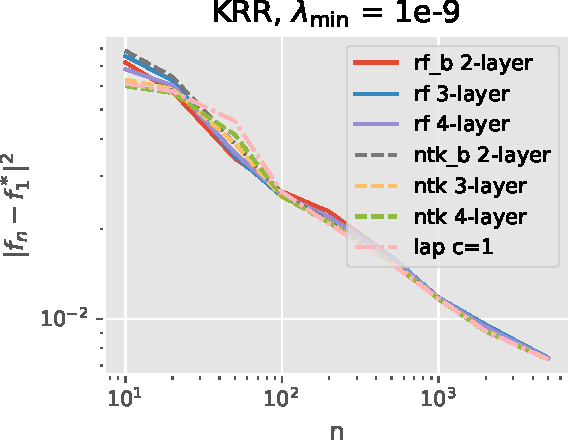
\includegraphics[width=.32\textwidth]{figures/full_kernel_9.pdf}
	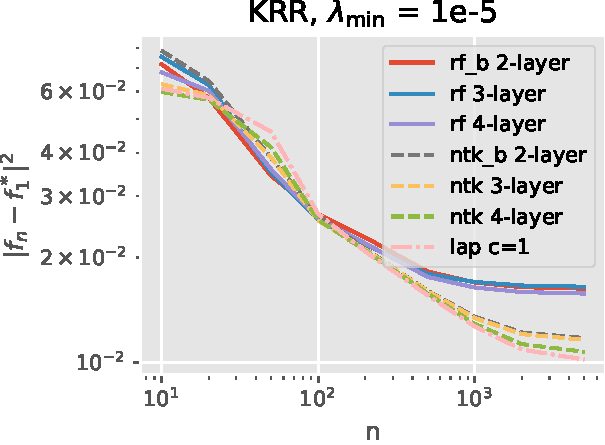
\includegraphics[width=.343\textwidth]{figures/full_kernel_5.pdf}
	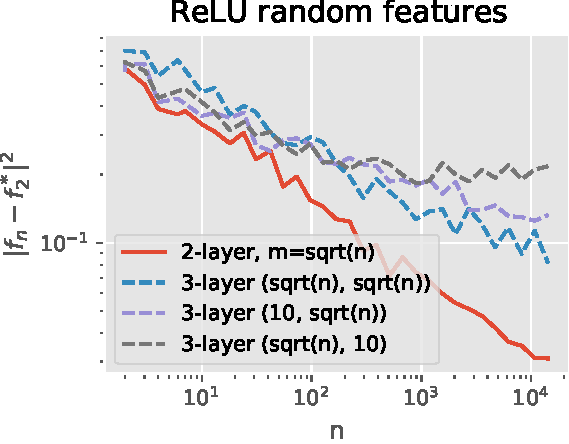
\includegraphics[width=.32\textwidth]{figures/relu_rf.pdf}
	\caption{(left, middle) expected squared error vs sample size~$n$ for kernel ridge regression estimators with different kernels on~$f_1^*$ and with two different budgets on optimization difficulty~$\lambda_{\min}$ (the minimum regularization parameter allowed). (right) ridge regression with one or two layers of random ReLU features on~$f_2^*$, with different scalings of the number of ``neurons'' at each layer in terms of~$n$.}
	\label{fig:synthetic}
\end{figure}


\paragraph{MNIST and Fashion-MNIST.}
In Table~\ref{tab:mnist_acc}, we consider the image classification datasets MNIST and Fashion-MNIST, which both consist of 60k training and 10k test images of size 28x28 with 10 output classes.
We evaluate one-versus-all classifiers obtained by using kernel ridge regression by setting~$y=0.9$ for the correct label and~$y=-0.1$ otherwise.
We train on random subsets of 50k examples and use the remaining 10k examples for validation.
We find that test accuracy is comparable for different numbers of layers in RF or NTK kernels, with a slightly poorer performance for the two-layer case likely due to parity constraints, in agreement with our theoretical result that the decay is the same for different~$L$.
There is a small decrease in accuracy for growing~$L$, which may reflect changes in the decay constants or numerical errors when composing kernels.
The slightly better performance of RF compared to NTK may suggest that these problems are relatively easy (\eg, the regression function is smooth), so that a faster decay is preferable due to better adaptivity to smoothness.

\begin{table}[t]
\caption{Test accuracies on MNIST (left) and Fashion-MNIST (right) for RF and NTK kernels with varying numbers of layers~$L$.
We use kernel ridge regression on 50k samples, with~$\lambda$ optimized on a validation set of size 10k, and report mean and standard errors across 5 such random splits of the 60k training samples.
For comparison, the Laplace kernel with~$c=1$ yields accuracies $98.39 \pm 0.02$ on MNIST and $90.38 \pm 0.06$ on F-MNIST.}
\label{tab:mnist_acc}
\centering

MNIST \hspace{4cm} F-MNIST
\vspace{0.1cm}
\small

\begin{tabular}{ | c |  c |  c |  }
\hline
L &  RF & NTK \\ \hline
2  & 98.60 $\pm$ 0.03 
 & 98.49 $\pm$ 0.02 
\\ 
3  & 98.67 $\pm$ 0.03 
 & 98.53 $\pm$ 0.02 
\\ 
4  & 98.66 $\pm$ 0.02 
 & 98.49 $\pm$ 0.01 
\\ 
5  & 98.65 $\pm$ 0.04 
 & 98.46 $\pm$ 0.02 
\\ 
\hline
\end{tabular}
~~
\begin{tabular}{ | c |  c |  c |  }
\hline
L &  RF & NTK \\ \hline
2  & 90.75 $\pm$ 0.11 
 & 90.65 $\pm$ 0.07 
\\ 
3  & 90.87 $\pm$ 0.16 
 & 90.62 $\pm$ 0.08 
\\ 
4  & 90.89 $\pm$ 0.13 
 & 90.55 $\pm$ 0.07 
\\ 
5  & 90.88 $\pm$ 0.08 
 & 90.50 $\pm$ 0.05 
\\ 
\hline
\end{tabular}

\end{table}



\section{Discussion}
%!TEX root = main.tex

In this paper, we have analyzed the approximation properties of deep networks in kernel regimes, by studying eigenvalue decays of integral operators through differentiability properties of the kernel function.
In particular, the decay is governed by the form of the function's (generalized) power series expansion around~$\pm 1$, which remains the same for kernels arising from fully-connected ReLU networks of varying depths.
This result suggests that the kernel approach is unsatisfactory for understanding the power of depth in fully-connected networks.
In particular, it highlights the need to incorporate other regimes in the study of deep networks, such as the mean field regime~\citep{chizat2018global,mei2018mean}, and other settings with hierarchical structure~\citep[see, \eg,][]{allen2020backward,chen2020towards}.
We note that our results do not rule out benefits of depth for other network architectures in kernel regimes; for instance, depth may improve stability properties of convolutional kernels~\citep{bietti2019group,bietti2019inductive}, and a precise study of approximation for such kernels and its dependence on depth would also be of interest.


\subsubsection*{Acknowledgments}
The authors would like to thank David Holzmüller for finding an error in an earlier version of the paper, which led us to include the new assumption on differentiation of asymptotic expansions in Theorem~\ref{thm:decay}.
This work was funded in part by the French government under management of Agence Nationale
de la Recherche as part of the ``Investissements d’avenir'' program, reference ANR-19-P3IA-0001
(PRAIRIE 3IA Institute). We also acknowledge support of the European Research Council (grant
SEQUOIA 724063).

\bibliography{full,bibli}
\bibliographystyle{iclr2021_conference}

\appendix
\section{Background on Spherical Harmonics}
\label{sec:appx_background}
%!TEX root = main.tex


In this section, we provide some background on spherical harmonics needed for our study of approximation.
See~\citep{costas2014spherical,atkinson2012spherical,ismail2005classical} for references, as well as~\citep[Appendix D]{bach2017breaking}.
We consider inputs on the $d-1$ sphere~$\mathbb S^{\dmone} = \{x \in \R^d, \|x\| = 1\}$.

We recall some properties of the spherical harmonics~$Y_{k,j}$ introduced in Section~\ref{sub:dp_kernel_approx}.
For~$j = 1, \ldots, N(d, k)$, where~$N(d,k) = \frac{2k + d - 2}{k} {k + d - 3 \choose d - 2}$, the spherical harmonics~$Y_{k,j}$ are homogeneous harmonic polynomials of degree~$k$ that are orthonormal with respect to the uniform distribution~$\tau$ on the~$\dmone$ sphere.
The degree~$k$ plays the role of an integer frequency, as in Fourier series, and the collection~$\{Y_{k,j}, k \geq 0, j = 1, \ldots, N(d,k)\}$ forms an orthonormal basis of~$L^2(\Sbb^{\dmone}, d\tau)$.
As with Fourier series, there are tight connections between decay of coefficients in this basis w.r.t.~$k$, and regularity/differentiability of functions, in this case differentiability on the sphere.
This follows from the fact that spherical harmonics are eigenfunctions of the Laplace-Beltrami operator on the sphere~$\Delta_{\Sbb^{d-1}}$~\citep[see][Proposition 4.5]{costas2014spherical}:
\begin{equation}
\label{eq:laplace_beltrami}
\Delta_{\Sbb^{d-1}} Y_{k,j} = -k(k+d-2)Y_{k,j}.
\end{equation}

For a given frequency~$k$, we have the following addition formula:
\begin{equation}
\label{eq:spherical_addition}
\sum_{j=1}^{N(d, k)} Y_{k,j}(x) Y_{k,j}(y) = N(d, k) P_k( x^\top y ),
\end{equation}
where~$P_k$ is the $k$-th Legendre polynomial in dimension~$d$ (also known as Gegenbauer polynomial when using a different scaling),
given by the Rodrigues formula:
\begin{equation}
\label{eq:rodrigues}
P_k(t) = (-1/2)^k \frac{\Gamma(\frac{d-1}{2})}{\Gamma(k + \frac{d-1}{2})} (1 - t^2)^{(3-d)/2}
	\left(\frac{d}{dt}\right)^k (1 - t^2)^{k+(d-3)/2}.
\end{equation}
Note that these may also be expressed using the hypergeometric function~$\pFq{2}{1}$~\citep[see, \eg,][Section 4.5]{ismail2005classical}, an expression we will use in proof of Theorem~\ref{thm:decay} (see the proof of Lemma~\ref{lemma:phi_nu}).

The polynomials~$P_k$ are orthogonal in~$L^2([-1, 1], d\nu)$ where the measure $d \nu$ is given by the weight function
$d \nu(t) = (1 - t^2)^{(d-3)/2}dt$, and we have
\begin{equation}
\label{eq:legendre_norm}
\int_{-1}^1 P_k^2(t) (1 - t^2)^{(d-3)/2}dt = \frac{\omega_{d-1}}{\omega_{d-2}} \frac{1}{N(d,k)},
\end{equation}
where~$\omega_{p-1} = \frac{2 \pi^{p/2}}{\Gamma(p/2)}$ denotes the surface of the sphere~$\mathbb S^{p-1}$ in~$p$ dimensions.
Using the addition formula~\eqref{eq:spherical_addition} and orthogonality of spherical harmonics, we can show
\begin{equation}
\label{eq:legendre_dp}
\int P_j( w^\top x ) P_k( w^\top y ) d \tau(w) = \frac{\delta_{jk}}{N(d,k)} P_k( x^\top y )
\end{equation}
We will use two other properties of Legendre polynomials, namely the following recurrence relation~\cite[Eq. 4.36]{costas2014spherical}
\begin{equation}
\label{eq:legendre_rec}
t P_k(t) = \frac{k}{2k + d - 2} P_{\kmone}(t) + \frac{k + d - 2}{2k + d - 2} P_{k+1}(t),
\end{equation}
for $k \geq 1$, and for $k = 0$ we simply have $t P_0(t) = P_1(t)$, as well as the differential equation
~\citep[see, \eg,][Proposition 4.20]{costas2014spherical}:
\begin{equation}
\label{eq:pk_ode}
(1 - t^2) P_k''(t) + (1 - d) t P_k'(t) + k(k + d - 2) P_k(t) = 0.
\end{equation}

The Funk-Hecke formula is helpful for computing Fourier coefficients in the basis of spherical harmonics in terms of
Legendre polynomials: for any~$j = 1, \ldots, N(d, k)$, we have
\begin{equation}
\label{eq:funk_hecke}
\int f(x^\top y) Y_{k,j}(y) d \tau(y) = \frac{\omega_{d-2}}{\omega_{d-1}} Y_{k,j}(x) \int_{-1}^1 f(t) P_k(t) (1 - t^2)^{(d-3)/2} dt.
\end{equation}
For example, we may use this to obtain decompositions of dot-product kernels by computing Fourier coefficients of functions~$\kappa(\langle x, \cdot \rangle)$.
Indeed, denoting
\begin{equation*}
\mu_k = \frac{\omega_{d-2}}{\omega_{d-1}} \int_{-1}^1 \kappa(t) P_k(t) (1 - t^2)^{(d-3)/2}dt,
\end{equation*}
writing the decomposition of~$\kappa(\langle x, \cdot \rangle)$ using~\eqref{eq:funk_hecke} leads to the following Mercer decomposition of the kernel:
\begin{equation}
\label{eq:mercer}
\kappa(x^\top y) = \sum_{k=0}^\infty \mu_k \sum_{j=1}^{N(d,k)} Y_{k,j}(x) Y_{k,j}(y) = \sum_{k=0}^\infty \mu_k N(d,k) P_k(x^\top y).
\end{equation}




\section{Proof of Theorem~\ref{thm:decay}}
\label{sec:appx_thm_proof}
%!TEX root = main.tex

The proof of Theorem~\ref{thm:decay}, stated below in full as Theorem~\ref{thm:decay_full}, proceeds as follows.
We first derive an upper bound on the decay of~$\kappa$ of the form~$k^{-d-2 \nu + 3}$ (Lemma~\ref{lemma:diff_decay}), which is weaker than the desired~$k^{-d-2 \nu + 1}$, by exploiting regularity properties of~$\kappa$ through integration by parts.
The goal is then to apply this result on a function~$\tilde \kappa = \kappa - \psi$, where~$\psi$ is a function that allows us to ``cancel'' the leading terms in the expansions of~$\kappa$, while being simple enough that it allows a precise estimate of its decay.
In the proof of Theorem~\ref{thm:decay_full}, we follow this strategy by considering~$\psi$ as a sum of functions of the form~$t \mapsto (1 - t^2)^\nu$ and~$t \mapsto t(1 - t^2)^\nu$, for which we provide a precise computation of the decay in Lemma~\ref{lemma:phi_nu}.


\paragraph{Decay upper bound through regularity.}
We begin by establishing a weak upper bound on the decay of~$\kappa$ (Lemma~\ref{lemma:diff_decay}) by leveraging its regularity up to the terms of order~$(1 - t^2)^\nu$.
This is achieved by iteratively applying the following integration by parts lemma, which is conceptually similar to integrating by parts on the sphere by leveraging the spherical Laplacian relation~\eqref{eq:laplace_beltrami} in Appendix~\ref{sec:appx_background}, but directly uses properties of~$\kappa$ and of Legendre polynomials instead (namely, the differential equation~\eqref{eq:pk_ode}).
We note that the final statement in Theorem~\ref{thm:decay} on infinitely differentiable~$\kappa$ directly follows from Lemma~\ref{lemma:diff_decay}.

\begin{lemma}[Integration by parts lemma]
\label{lemma:ode_recursion}
Let~$\kappa: [-1,1] \to \R$ be a function that is~$C^\infty$ on~$(-1,1)$ and such that~$\kappa'(t) (1-t^2)^{1+\frac{d-3}{2}} = O(1)$. We have
\begin{align}
\int_{-1}^1 \kappa(t) P_k(t) (1-t^2)^{\frac{d-3}{2}} dt &= \frac{1}{k(k+d-2)} \Big( -\kappa(t)(1 - t^2)^{1 + \frac{d-3}{2}} P_k'(t) \Big|_{-1}^1 \\
	&\quad+ \kappa'(t) (1 - t^2)^{1 + \frac{d-3}{2}} P_k(t) \Big|_{-1}^1  + \int_{-1}^1 \tilde \kappa(t) P_k(t) (1 - t^2)^{(d-3)/2} dt \Big),
\end{align}
with~$\tilde \kappa(t) = -\kappa''(t)(1 - t^2) + (d-1)t \kappa'(t)$.
\end{lemma}
\begin{proof}
In order to perform integration by parts, we use the following differential equation satisfied by Legendre polynomials~\citep[see, \eg,][Proposition 4.20]{costas2014spherical}:
\begin{equation}
(1 - t^2) P_k''(t) + (1 - d) t P_k'(t) + k(k + d - 2) P_k(t) = 0.
\end{equation}
Using this equation, we may write for~$k \geq 1$,
\begin{align}
\label{eq:pk_ipp}
\int_{-1}^1 \kappa(t) P_k(t) (1 - t^2)^{(d-3)/2} dt 
	&= \frac{1}{k(k+d-2)} \Big( (d-1) \int t \kappa(t) P_k'(t) (1 - t^2)^{\frac{d-3}{2}} dt \\
		&\qquad- \int \kappa(t) P_k''(t) (1 - t^2)^{1 + \frac{d-3}{2}}dt \Big).
\end{align}
We may integrate the second term by parts using
\begin{align}
\frac{d}{dt} \left( \kappa(t) (1 - t^2)^{1 + \frac{d-3}{2}} \right)
	&= \kappa'(t) (1 - t^2)^{1 + \frac{d-3}{2}} - 2t(1 + (d-3)/2) \kappa(t) (1 - t^2)^{\frac{d-3}{2}} \nonumber\\
	&= \kappa'(t) (1 - t^2)^{1 + \frac{d-3}{2}} - (d-1) t \kappa(t)(1 - t^2)^{\frac{d - 3}{2}} \label{eq:ipp_diff}.
\end{align}
Noting that the first term in~\eqref{eq:pk_ipp} cancels out with the integral resulting from the second term in~\eqref{eq:ipp_diff}, we then obtain
\begin{align*}
\int_{-1}^1 \kappa(t) P_k(t) (1 - t^2)^{(d-3)/2} dt &= \frac{1}{k(k+d-2)} \Big( -\kappa(t)(1 - t^2)^{1 + \frac{d-3}{2}} P_k'(t) \Big|_{-1}^1  \\
	&\qquad + \int_{-1}^1 \kappa'(t) (1 - t^2)^{1 + \frac{d-3}{2}} P_k'(t) dt \Big).
\end{align*}
Integrating by parts once more, the second term becomes
\begin{align}
\int_{-1}^1 \kappa'(t) (1 - t^2)^{1 + \frac{d-3}{2}} P_k'(t) dt &= \kappa'(t) (1 - t^2)^{1 + \frac{d-3}{2}} P_k(t) \Big|_{-1}^1 \nonumber \\
	&\quad- \int_{-1}^1 (\kappa''(t)(1 - t^2) - (d-1)t \kappa'(t)) P_k(t) (1 - t^2)^{(d-3)/2} dt.
\end{align}
The desired result follows.
\end{proof}

\begin{lemma}[Weak upper bound on the decay]
\label{lemma:diff_decay}
Let~$\kappa: [-1,1] \to \R$ be a function that is~$C^\infty$ on~$(-1,1)$ and has the following expansions around~$\pm 1$ on its derivatives:
\begin{align}
\kappa^{(j)}(t) &= p_{j,1}(1-t) + O((1-t)^{\nu-j}) \\
\kappa^{(j)}(t) &= p_{j,-1}(1+t) + O((1+t)^{\nu-j}), 
\end{align}
for~$t \in [-1, 1]$ and $j \geq 0$, where~$p_{j,1}, p_{j,-1}$ are polynomials and~$\nu$ may be non-integer.
Then the Legendre coefficients~$\mu_k(\kappa)$ of~$\kappa$ given in~\eqref{eq:mu_k} satisfy
\begin{equation}
\mu_k(\kappa) = O(k^{-d-2 \nu + 3}).
\end{equation}
\end{lemma}

\begin{proof}
Let~$f_0 := \kappa$ and for~$j \geq 1$
\begin{align}
f_j(t) := -f_{j-1}''(t)(1 - t^2) + (d-1) f_{j-1}'(t).
\end{align}
Then~$f_j$ is~$C^\infty$ on~$(-1,1)$ and has similar expansions to~$\kappa$ of the form
\begin{align}
f_j(t) &= q_{j,1}(1-t) + O((1-t)^{\nu-j}) \\
f_j(t) &= q_{j,-1}(1+t) + O((1+t)^{\nu-j}),
\end{align}
for some polynomials~$q_{j,\pm 1}$.
We may apply Lemma~\ref{lemma:ode_recursion} repeatedly as long as the terms in brackets vanish, until we obtain, for~$j = \lceil \nu + \frac{d-3}{2} \rceil - 1$,
\begin{align*}
\int_{-1}^1 &\kappa(t) P_k(t) (1 - t^2)^{(d-3)/2} dt \\
	&= \frac{1}{(k(k+d-2))^{j+1}}
\left( f_j'(t) (1 - t^2)^{1 + \frac{d-3}{2}} P_k(t) \Big|_{-1}^1 + \int_{-1}^1 f_{j+1}(t) P_k(t) (1 - t^2)^{(d-3)/2} dt \right).
\end{align*}
Given our choice for~$j$, we have $f_j'(t) (1 - t^2)^{1 + \frac{d-3}{2}} = O(1)$, and $f_{j+1}(t) (1 - t^2)^{(d-3)/2} = O((1-t^2)^{-1+ \epsilon})$ for some~$\epsilon > 0$. Since~$P_k(t) \in [-1, 1]$ for any~$t \in [-1, 1]$, we obtain $\mu_k(\kappa) = O(k^{-2(j+1)}) = O(k^{-d-2 \nu+3})$.
\end{proof}

\paragraph{Precise decay for simple function.}
We now provide precise decay estimates for functions of the form~$t \mapsto (1 - t^2)^\nu$ and~$t \mapsto t(1 - t^2)^\nu$, which will lead to the dominant terms in the decomposition of~$\kappa$ in the main theorem.


\begin{lemma}[Decay for simple functions~$\phi_\nu$ and~$\bar \phi_\nu$]
\label{lemma:phi_nu}
Let $\phi_\nu(t) = (1 - t^2)^\nu$, with~$\nu > 0$ non-integer, and let~$\mu_k(\phi_\nu)$ denote its Legendre coefficients in~$d$ dimensions given by~$\frac{\omega_{d-2}}{\omega_{d-1}}\int_{-1}^1 (1 - t^2)^{\nu + (d-3)/2} P_k(t) dt$.
We have
\begin{itemize}
	\item $\mu_k(\phi_\nu) = 0$ if~$k$ is odd
	\item $\mu_k(\phi_\nu) \sim C(d,\nu) k^{-d-2 \nu - 1}$ for~$k$ even, $k \to \infty$, with~$C(d,\nu)$ a constant.
\end{itemize}
Analogously, let $\bar \phi_\nu(t) := t(1 - t^2)^{\nu}$. We have
\begin{itemize}
	\item $\mu_k(\bar \phi_\nu) = 0$ if~$k$ is even
	\item $\mu_k(\bar \phi_\nu) \sim C(d,\nu) k^{-d-2 \nu - 1}$ for~$k$ odd, $k \to \infty$, with~$C(d,\nu)$ a constant.
\end{itemize}

\end{lemma}
\begin{proof}
We recall the following representation of Legendre polynomials based on the hypergeometric function~\citep[\eg,][Section 4.5]{ismail2005classical}:\footnote{Here we normalize such that~$P_k(1)=1$ as is standard for Legendre polynomials, in contrast to~\citep{ismail2005classical} where the standard Jacobi/Gegenbauer normalization is used.}
\begin{equation}
P_k(t) = \pFq{2}{1}(-k,k+d-2;(d-1)/2;(1-t)/2),
\end{equation}
where the hypergeometric function is given in its generalized form by
\begin{equation}
\pFq{p}{q}(a_1, \ldots, a_p;b_1, \ldots, b_q;x)
= \sum_{s=0}^\infty \frac{(a_1)_s \cdots (a_p)_s}{(b_1)_s \cdots (b_q)_s} \frac{x^s}{s!},
\end{equation}
where~$(a)_s = \Gamma(a+s)/\Gamma(a)$ is the rising factorial or Pochhammer symbol.

Using the above definitions and the integral representation of Beta functions, we then have
\begin{align*}
\int_{-1}^1 (1-t^2)^{\nu + \frac{d-3}{2}} P_k(t) dt
	&= 2^{2 \nu + d - 3} \int_{-1}^1 \left(\frac{1-t}{2}\right)^{\nu + \frac{d-3}{2}} \left(\frac{1+t}{2}\right)^{\nu + \frac{d-3}{2}} P_k(t) dt \\
	&= 2^{2 \nu + d - 3} \sum_{s=0}^k \frac{(-k)_s (d-2+k)_s}{\left( \frac{d-1}{2}\right)_s s!} \int_{-1}^1 \left(\frac{1-t}{2}\right)^{\nu + \frac{d-3}{2} + s} \left(\frac{1+t}{2}\right)^{\nu + \frac{d-3}{2}} dt \\
	&= 2^{2 \nu + d - 2} \sum_{s=0}^k \frac{(-k)_s (d-2+k)_s}{\left( \frac{d-1}{2}\right)_s s!} \int_{0}^1 \left(1-x\right)^{\nu + \frac{d-3}{2} + s} x^{\nu + \frac{d-3}{2}} dx \\
	&= 2^{2 \nu + d - 2} \sum_{s=0}^k \frac{(-k)_s (d-2+k)_s}{\left( \frac{d-1}{2}\right)_s s!} \frac{\Gamma(\nu +s + \frac{d-1}{2}) \Gamma(\nu + \frac{d-1}{2})}{\Gamma(2 \nu + s + d - 1)} \\
	&= 2^{2 \nu + d - 2} \frac{\Gamma(\nu + \frac{d-1}{2})^2}{\Gamma(2 \nu + d - 1)} \sum_{s=0}^k \frac{(-k)_s (d-2+k)_s (\nu + \frac{d-1}{2})_s}{\left( \frac{d-1}{2}\right)_s (2 \nu + d - 1)_s s!} \\
	&= 2^{2 \nu + d - 2} \frac{\Gamma(\nu + \frac{d-1}{2})^2}{\Gamma(2 \nu + d - 1)} \pFq{3}{2}\left(\begin{matrix}
		-k,k+d-2, \nu + (d-1)/2 \\ (d-1)/2, 2 \nu + d - 1
	\end{matrix}\Big| 1 \right).
\end{align*}

Now, we use Watson's theorem~\citep[\eg,][Eq.~(1.4.12)]{ismail2005classical}, which states that
\begin{equation}
\pFq{3}{2}\left(\begin{matrix}
		a,b,c \\ (a + b + 1)/2, 2c
	\end{matrix}\Big|1 \right) = \frac{\Gamma(\frac{1}{2}) \Gamma(c + \frac{1}{2}) \Gamma(\frac{a+b+1}{2}) \Gamma(c + \frac{1 - a - b}{2})}{\Gamma(\frac{a+1}{2})\Gamma(\frac{b+1}{2}) \Gamma(c + \frac{1-a}{2})}.
\end{equation}

We remark that with~$a=-k, b=k+d-2, c=\nu + (d-1)/2$, our expression above is of the form of Watson's theorem, and we may thus evaluate~$\mu_k$ in closed form.
Indeed, we have
\begin{align}
\pFq{3}{2}\left(\begin{matrix}
		-k,k+d-2, \nu + (d-1)/2 \\ (d-1)/2, 2 \nu + d - 1
	\end{matrix}\Big| 1 \right)
	&= \frac{\Gamma(\frac{1}{2}) \Gamma(\nu + \frac{d}{2}) \Gamma(\frac{d-1}{2}) \Gamma(\nu + 1)}{\Gamma(\frac{1-k}{2}) \Gamma(\frac{d+k-1}{2}) \Gamma(\nu + \frac{k}{2} + \frac{d}{2}) \Gamma(\nu + 1 - \frac{k}{2})}.
\end{align}
When~$k$ is odd, then~$(1-k)/2$ is a non-positive integer so that the denominator is infinite and thus~$\mu_k$ vanishes. We assume from now on that~$k$ is even, making the denominator is finite.
Using the following relation, for~$\epsilon \notin \Z$ and an integer~$n$:
\begin{equation}
\frac{\Gamma(1+\epsilon)}{\Gamma(\epsilon - n)} = \epsilon(\epsilon-1) \cdots (\epsilon - n) = (-1)^{n-1} \frac{\Gamma(n+1- \epsilon)}{\Gamma(-\epsilon)},
\end{equation}
we may then rewrite
\begin{align}
\pFq{3}{2}\left(\begin{matrix}
		-k,k+d-2, \nu + (d-1)/2 \\ (d-1)/2, 2 \nu + d - 1
	\end{matrix}\Big| 1 \right)
	&= \frac{\Gamma(\nu + \frac{d}{2}) \Gamma(\frac{d-1}{2}) \Gamma(\nu + 1)}{\Gamma(-\frac{1}{2}) \Gamma(\nu + 2) \Gamma(-\nu - 1)} \frac{\Gamma(\frac{k + 1}{2}) \Gamma(\frac{k}{2} - \nu) }{\Gamma(\frac{d+k-1}{2}) \Gamma(\nu + \frac{k}{2} + \frac{d}{2})}.
\end{align}
When~$k \to \infty$, Stirling's formula~$\Gamma(x) \sim x^{x - \frac{1}{2}} e^{-x} \sqrt{2 \pi}$ yields the equivalent
\begin{equation}
\frac{\Gamma(\frac{k + 1}{2}) \Gamma(\frac{k}{2} - \nu) }{\Gamma(\frac{d+k-1}{2}) \Gamma(\nu + \frac{k}{2} + \frac{d}{2})} \sim \left(\frac{k}{2} \right)^{-d-2 \nu + 1}.
\end{equation}
This yields
\begin{equation}
\mu_k \sim C(d,\nu) k^{-d-2 \nu + 1},
\end{equation}
with
\begin{align}
C(d,\nu) &= 2^{2 \nu + d - 2} \frac{\omega_{d-2}}{\omega_{d-1}} \frac{\Gamma(\nu + \frac{d-1}{2})^2}{\Gamma(2 \nu + d - 1)} \frac{\Gamma(\nu + \frac{d}{2}) \Gamma(\frac{d-1}{2}) \Gamma(\nu + 1)}{\Gamma(-\frac{1}{2}) \Gamma(\nu + 2) \Gamma(-\nu - 1)} (1/2)^{-d-2 \nu + 1}.
\end{align}

\paragraph{Decay for~$\bar \phi_\nu$.}
The decay for~$\bar \phi_\nu$ follows from the decay of~$\phi_\nu$ and the recurrence relation~\citep[][Eq.~(4.36)]{costas2014spherical}
\begin{equation}
t P_k(t) = \frac{k}{2k + d - 2}P_{k-1}(t) + \frac{k+d - 2}{2k + d - 2} P_{k+1}(t),
\end{equation}
which ensures the same decay with a change parity.
\end{proof}



\paragraph{Final theorem.}
We are now ready to prove our main theorem, which differs from the simplified statement of Theorem~\ref{thm:decay} by the technical assumption that only a finite number~$r$ of terms of order between~$\nu$ and~$\nu + 1$ are present in the series expansions around~$\pm 1$.

\begin{theorem}[Main theorem, full version]
\label{thm:decay_full}
Let~$\kappa: [-1,1] \to \R$ be a function that is~$C^\infty$ on~$(-1,1)$ and has the following expansions around~$\pm 1$:
\begin{align}
\kappa(t) &= p_1(1-t) + \sum_{j=1}^r c_{j,1} (1-t)^{\nu_j} + O((1-t)^{\nu_1 + 1 + \epsilon}) \\
\kappa(t) &= p_{-1}(1+t) + \sum_{j=1}^r c_{j,-1} (1+t)^{\nu_j} + O((1+t)^{\nu_1 + 1 + \epsilon}),
\end{align}
for~$t \in [-1, 1]$, where~$p_1, p_{-1}$ are polynomials and~$0 < \nu_1 < \ldots < \nu_r$ are not integers and $0 < \epsilon < \nu_2 - \nu_1$.
We also assume that the derivatives~$\kappa^{(s)}$ of~$\kappa$ have the following expansions:
\begin{align}
\kappa^{(s)}(t) &= p_{s,1}(1-t) + (-1)^s\sum_{j=1}^r c_{j,1} \frac{\Gamma(\nu_j + 1)}{\Gamma(\nu_j + 1 - s)} (1-t)^{\nu_j-s} + O((1-t)^{\nu_1 + 1 + \epsilon - s}) \\
\kappa^{(s)}(t) &= p_{s,-1}(1+t) + \sum_{j=1}^r c_{j,-1} \frac{\Gamma(\nu_j + 1)}{\Gamma(\nu_j + 1 - s)} (1+t)^{\nu_j-s} + O((1+t)^{\nu_1 + 1 + \epsilon - s}),
\end{align}
for some polynomials~$p_{s,\pm 1}$.
Then we have, for an absolute constant~$C(d,\nu_1)$ depending only on~$d$ and~$\nu_1$,
\begin{itemize}[noitemsep]
	\item For~$k$ even, if~$c_{\nu_1,1} \ne -c_{1,-1}$: $\mu_k \sim (c_{1,1} + c_{1,-1}) C(d,\nu_1) k^{-d-2 \nu_1 + 1}$;
	\item For~$k$ even, if~$c_{1,1} = -c_{1,-1}$: $\mu_k = o(k^{-d-2 \nu_1 + 1})$;
	\item For~$k$ odd, if~$c_{1,1} \ne c_{1,-1}$: $\mu_k \sim (c_{1,1} - c_{1,-1}) C(d,\nu_1) k^{-d-2 \nu_1 + 1}$.
	\item For~$k$ odd, if~$c_{1,1} = c_{1,-1}$: $\mu_k =o(k^{-d-2 \nu_1 + 1})$.
\end{itemize}
\end{theorem}

\begin{proof}
Define the functions
\begin{align}
\psi_j(t) &= c_{j,1} \frac{\phi_{\nu_j}(t) + \bar \phi_{\nu_j}(t)}{2^{\nu_j + 1}} + c_{j,-1} \frac{\phi_{\nu_j}(t) - \bar \phi_{\nu_j}(t)}{2^{\nu_j + 1}} \label{eq:psij_def} \\
	&= \frac{c_{j,1} + c_{j,-1}}{2^{\nu_j + 1}} \phi_{\nu_j}(t) + \frac{c_{j,1} - c_{j,-1}}{2^{\nu_j + 1}} \bar \phi_{\nu_j}(t),
\end{align}
for~$j = 1, \ldots, r$, where~$\phi_{\nu}, \bar \phi_\nu$ are defined in Lemma~\ref{lemma:phi_nu}.
We have the asymptotic expansions:\footnote{These are obtained by writing $\psi_j(t) = (a + bt) (1 + t)^\nu (1 - t)^\nu$ and computing, \eg, the first two terms in the analytic expansion of~$t \mapsto (a + bt) (1 + t)^\nu$ around 1.}
\begin{align*}
\psi_1(t) &= c_{1,1} (1 - t)^{\nu_1} - \frac{(1 + \nu_1)c_{1,1} + c_{1,-1}}{2} (1 - t)^{\nu_1 + 1} + O((1 - t)^{\nu_1 + 1 + \epsilon}) \\
\psi_1(t) &= c_{1,-1} (1 + t)^{\nu_1} + \frac{c_{1,1} - (1 + \nu) c_{1,-1}}{2} (1 + t)^{\nu_1 + 1} + O((1 + t)^{\nu_1 + 1 + \epsilon}),
\end{align*}
and for~$j \geq 2$,
\begin{align*}
\psi_j(t) &= c_{j,1} (1 - t)^{\nu_j} + O((1 - t)^{\nu_1 + 1 + \epsilon}) \\
\psi_j(t) &= c_{j,-1} (1 + t)^{\nu_j} + O((1 + t)^{\nu_1 + 1 + \epsilon}).
\end{align*}
Define additionally~$\psi_{r+1}$ the same way as the other~$\psi_j$, with~$\nu_{r+1} = \nu_1 + 1$, $c_{r+1,1} = ((1 + \nu_1)c_{1,1} + c_{1,-1})/2$, and~$c_{r+1,-1} = -(c_{1,1} - (1 + \nu) c_{1,-1})/2$, which satisfies a similar asymptotic expansion as the above ones for~$j \geq 2$.
One can check that the derivatives of the~$\psi_j$ can be expanded with the derivatives of the expansions above.
Then, defining $\tilde \kappa = \kappa - \sum_{j=1}^{r+1} \psi_j$, we have for~$s \geq 0$,
\begin{align}
\tilde \kappa^{(s)}(t) &= p_{s,1}(1-t) + O((1-t)^{\nu_1 + 1 + \epsilon - s}) \\
\tilde \kappa^{(s)}(t) &= p_{s,-1}(1+t) + O((1+t)^{\nu_1 + 1 + \epsilon - s}).
\end{align}
The functions~$\psi_j$ satisfy
\begin{equation}
\mu_k(\psi_j) = \begin{cases}
	\frac{c_{j,1} + c_{j,-1}}{2^{\nu_j + 1}} \mu_k(\phi_{\nu_j}), &\text{ if $k$ even,}\\
	\frac{c_{j,1} - c_{j,-1}}{2^{\nu_j + 1}} \mu_k(\bar \phi_{\nu_j}), &\text{ if $k$ odd.}\\
\end{cases}
\end{equation}
By Lemma~\ref{lemma:diff_decay}, we have
\begin{align}
\mu_k(\kappa) &= \mu_k(\tilde \kappa) + \sum_{j=1}^r \mu_k(\psi_j) \\
	&= \sum_{j=1}^r \mu_k(\psi_j) + O(k^{-d - 2 (\nu_1 + 1 + \epsilon) + 3}) \\
	&= \sum_{j=1}^r \mu_k(\psi_j) + o(k^{-d - 2 \nu_{1} + 1}).
\end{align}
The result then follows from Lemma~\ref{lemma:phi_nu}, with a constant~$C(d, \nu_1) / 2^{\nu_1 + 1}$, where~$C(d, \nu_1)$ is given by the proof of Lemma~\ref{lemma:phi_nu}.
\end{proof}


\subsection{Dimension-free description}
\label{sub:appx_dimension_free}
While our above description of the RKHS depends on the dimension~$d$, in some cases a dimension-free description given by Taylor coefficients of the kernel~$\kappa$ at~$0$ may be useful,
for instance for the study of kernel methods in certain high-dimensional regimes~\citep[\eg,][]{el2010spectrum,ghorbani2019linearized,liang2019risk}.
Here we remark that such coefficients and their decay may be recovered from the Legendre coefficients in~$d$ dimensions, by taking high-dimensional limits~$d \to \infty$.
We illustrate this on the functions~$\phi_\nu(t) = (1 - t^2)^\nu$, for which Lemma~\ref{lemma:phi_nu} provides precise estimates of the Legendre coefficients~$\mu_{k,d}(\phi_\nu)$ in~$d$ dimensions (this only serves as an instructive illustration, since in this case Taylor coefficients may be computed directly through a power series expansion of~$\phi_\nu$ using the Binomial formula).
\begin{lemma}[Recovering Taylor coefficients of~$\phi_\nu$ through high-dimensional limits]
\label{lemma:bk_phinu}
Let~$b_k(\phi_\nu) := \frac{\phi_\nu^{(k)}}{k!}$ for some non-integer~$\nu > 0$. For~$k$ even, we have
\begin{equation*}
b_k(\phi_\nu) = C_\nu 2^k \frac{\Gamma(\frac{k + 1}{2}) \Gamma(\frac{k}{2} - \nu) }{\Gamma(k+1)},
\end{equation*}
for a constant~$C_\nu$ depending only on~$\nu$. This leads to an equivalent~$b_k \sim C_\nu' k^{- \nu - 1}$ for~$k \to \infty$ with~$k$ even.
\end{lemma}
\begin{proof}
Assume throughout that~$k$ is even.
Recall the expression of the Legendre coefficients~$\mu_{k,d}(\phi_\nu)$ of~$\phi_\nu$ in~$d$ dimensions (we include~$d$ as a subscript for more clarity here) from the proof of Lemma~\ref{lemma:phi_nu}:
\begin{align}
\mu_{k,d}(\phi_\nu) &= \frac{\omega_{d-2}}{\omega_{d-1}} \int_{-1}^1 \kappa(t) P_{k,d}(t) (1 - t^2)^{\frac{d-3}{2}} dt \\
	&= 2^{2 \nu + d - 2} \frac{\omega_{d-2}}{\omega_{d-1}} \frac{\Gamma(\nu + \frac{d-1}{2})^2}{\Gamma(2 \nu + d - 1)} \frac{\Gamma(\nu + \frac{d}{2}) \Gamma(\frac{d-1}{2}) \Gamma(\nu + 1)}{\Gamma(-\frac{1}{2}) \Gamma(\nu + 2) \Gamma(-\nu - 1)} \frac{\Gamma(\frac{k + 1}{2}) \Gamma(\frac{k}{2} - \nu) }{\Gamma(\frac{d+k-1}{2}) \Gamma(\nu + \frac{k}{2} + \frac{d}{2})}. \label{eq:mukd_phinu}
\end{align}

Now, note that when~$d$ is large enough compared to~$k$, we may use the Rodrigues formula~\eqref{eq:rodrigues} and integration by parts to obtain the following alternative expression:
\begin{equation*}
\mu_{k,d}(\phi_\nu) = 2^{-k} \frac{\omega_{d-2}}{\omega_{d-1}}  \frac{\Gamma(\frac{d-1}{2})}{\Gamma(k + \frac{d-1}{2})} \int_{-1}^1 \phi_\nu^{(k)}(t) (1 - t^2)^{k + \frac{d-3}{2}} dt
\end{equation*}
Following similar arguments to~\citet{ghorbani2019linearized}, we may then use dominated convergence to show:
\begin{equation*}
\frac{\Gamma(\frac{d}{2})}{\sqrt{\pi}\Gamma(\frac{d-1}{2})} \int_{-1}^1 \phi_\nu^{(k)}(t) (1 - t^2)^{k + \frac{d-3}{2}} dt \to \phi_\nu^{(k)}(0) \quad \text{ as }d \to \infty.
\end{equation*}
Indeed, $\frac{\Gamma(\frac{d}{2})}{\sqrt{\pi}\Gamma(\frac{d-1}{2})} (1 - t^2)^{(d-3)/2}$ is a probability density that approaches a Dirac mass at 0 when~$d \to \infty$.
This yields
\begin{equation*}
b_k(\phi_\nu) = \frac{\phi_\nu^{(k)}}{k!} = \lim_{d \to \infty} 2^{k} \frac{\omega_{d-1}}{\omega_{d-2}} \frac{\Gamma(\frac{d}{2})\Gamma(k + \frac{d-1}{2})}{\sqrt{\pi}\Gamma(\frac{d-1}{2}) \Gamma(\frac{d-1}{2}) \Gamma(k + 1)} \mu_{k,d}(\phi_\nu).
\end{equation*}
Plugging~\eqref{eq:mukd_phinu} and using Stirling's formula to take limits~$d \to \infty$ yields
\begin{equation*}
b_k(\phi_\nu) = C_\nu 2^k \frac{\Gamma(\frac{k + 1}{2}) \Gamma(\frac{k}{2} - \nu) }{\Gamma(k+1)},
\end{equation*}
where~$C_\nu$ only depends on~$\nu$. Using Stirling's formula once again yields the desired equivalent~$b_k(\phi_\nu) \sim C'_\nu k^{- \nu - 1}$ for~$k \to \infty$, $k$ even, with a different constant~$C'_\nu$.
\end{proof}

We note that a similar asymptotic equivalent holds for~$b_k(\bar \phi_\nu)$ for~$k$ odd.
The next result leverages this to derive asymptotic decays of~$b_k(\kappa)$ for any~$\kappa$ of the form~$\kappa(u) = \sum_{k \geq 0} b_k(\kappa) u^k$ satisfying similar conditions as in Theorem~\ref{thm:decay_full}.

\begin{corollary}[Taylor coefficients of~$\kappa$]
Let~$\kappa: [-1,1] \to \R$ be a function admitting a power series expansion~$\kappa(u) = \sum_{k \geq 0} b_k u^k$, with the following expansions around~$\pm 1$:
\begin{align}
\kappa(t) &= p_1(1-t) + \sum_{j=1}^r c_{j,1} (1-t)^{\nu_j} + O((1-t)^{\lceil\nu_1\rceil + 1}) \\
\kappa(t) &= p_{-1}(1+t) + \sum_{j=1}^r c_{j,-1} (1+t)^{\nu_j} + O((1+t)^{\lceil\nu_1\rceil + 1}),
\end{align}
for~$t \in [-1, 1]$, where~$p_1, p_{-1}$ are polynomials and~$0 < \nu_1 < \ldots < \nu_r$ are not integers and $0 < \epsilon < \nu_2 - \nu_1$.
Then we have, for an absolute constant~$C(\nu_1)$ depending only on~$\nu_1$,
\begin{itemize}[noitemsep]
	\item For~$k$ even, if~$c_{\nu_1,1} \ne -c_{\nu_1,-1}$: $b_k \sim (c_{\nu_1,1} + c_{\nu_1,-1}) C(\nu_1) k^{- \nu_1 - 1}$;
	\item For~$k$ even, if~$c_{\nu_1,1} = -c_{\nu_1,-1}$: $b_k = o(k^{- \nu_1 - 1})$;
	\item For~$k$ odd, if~$c_{\nu_1,1} \ne c_{\nu_1,-1}$: $b_k \sim (c_{\nu_1,1} - c_{\nu_1,-1}) C(\nu_1) k^{- \nu_1 - 1}$.
	\item For~$k$ odd, if~$c_{\nu_1,1} = c_{\nu_1,-1}$: $b_k =o(k^{- \nu_1 - 1})$.
\end{itemize}
\end{corollary}

\begin{proof}
As in the proof of Theorem~\ref{thm:decay_full}, we may construct a function~$\psi = \sum_j \alpha_j \phi_{\nu_j} + \bar \alpha_j \bar \phi_{\nu_j}$, with~$\alpha_1 = \frac{c_{1,1} + c_{1,-1}}{2^{\nu_1 + 1}}$, $\bar \alpha_1 = \frac{c_{1,1} - c_{1,-1}}{2^{\nu_1 + 1}}$ for~$j=1$, the other terms being of higher orders~$\nu_j > \nu_1$, such that~$\tilde \kappa := \kappa - \psi$ (which is also a power series with convergence radius $\geq 1$) satisfies
\begin{align}
\tilde \kappa(t) &= p_1(1-t) + O((1-t)^{\lceil\nu_1\rceil + 1}) \\
\tilde \kappa(t) &= p_{-1}(1+t) + O((1+t)^{\lceil\nu_1\rceil + 1}),
\end{align}
It follows that~$\tilde \kappa^{(\lceil\nu_1\rceil + 1)}(1)$ is bounded, so that the Taylor coefficients of~$\tilde \kappa$, denoted~$b_k(\tilde \kappa)$, satisfy
\begin{equation*}
b_k(\tilde \kappa) = o(k^{- \lceil\nu_1\rceil - 1}) = o(k^{- \nu_1 - 1}).
\end{equation*}
The result then follows from Lemma~\ref{lemma:bk_phinu} by using the decays of~$b_k(\phi_\nu)$ and~$b_k(\bar \phi_\nu)$.

\end{proof}

\section{Other Proofs}
\label{sec:appx_proofs}
%!TEX root = main.tex

In this section, we provide the proofs for results in Section~\ref{sub:extensions} related to obtaining power series expansions (with generalized exponents) of kernels arising from deep networks, which leads to the corresponding decays by Theorem~\ref{thm:decay}.
We note that for the kernels considered in this section, we can differentiate the expansions since the kernel function is $\Delta$-analytic~\citep[see][Theorem 7]{chen2020deep}, so that the technical assumption in Theorem~\ref{thm:decay} is verified.

\subsection{Proof of Corollary~\ref{cor:rf_decay}} % (fold)
\label{sub:rf_decay_proof}

\begin{proof}
Let~$\kappa^\ell := \underbrace{\kappa_1 \circ \cdots \circ \kappa_1}_{\ell-1 \text{ times}} = \kappa_{\RF}^\ell$. We have
\begin{equation*}
\kappa_1(1 - t) = 1 - t + c t^{3/2} + o(t^{3/2}), \quad c := \frac{2\sqrt{2}}{3 \pi}.
\end{equation*}
We now show by induction that~$\kappa^\ell(1 - t) = 1 - t + a_\ell t^{3/2} + o(t^{3/2})$, with~$a_\ell = (\ell - 1) c$.
This is obviously true for~$\ell = 2$ since~$\kappa^\ell = \kappa_1$, and for~$\ell \geq 3$ we have
\begin{align*}
\kappa^\ell(1 - t) &= \kappa_1(\kappa^{\ell-1}(1 - t)) \\
	&= \kappa_1(1 - t + a_{\ell-1} t^{3/2} + o(t^{3/2})) \\
	&= 1 - (t - a_{\ell-1} t^{3/2} + o(t^{3/2})) + c (t + O(t^{3/2}))^{3/2} + o(O(t)^{3/2}) \\
	&= 1 - t + a_{\ell-1} t^{3/2} + c t^{3/2}(1 + O(t^{1/2}))^{3/2} + o(t^{3/2}) \\
	&= 1 - t + a_{\ell-1} t^{3/2} + c t^{3/2}(1 + O(t^{1/2})) + o(t^{3/2}) \\
	&= 1 - t + a_\ell t^{3/2} + o(t^{3/2}),
\end{align*}
which proves the result.

Around~$-1$, we know that
\begin{equation*}
\kappa_1(-1 + t) = ct^{3/2} + o(t^{3/2}).
\end{equation*}
We then have~$\kappa^\ell(-1+t) = b_\ell + c_\ell t^{3/2} + o(t^{3/2})$, with~$0 \leq b_\ell < 1$ and~$0 < c_\ell \leq c$ (and the upper bound is strict for~$\ell \geq 3$).
Indeed, this is true for~$\ell=2$, and for~$\ell \geq 3$ we have, for~$t > 0$,
\begin{align*}
\kappa^\ell(-1+t) &= \kappa_1(\kappa^{\ell-1}(-1+t)) \\
	&= \kappa_1(b_{\ell-1} + c_{\ell-1} t^{3/2} + o(t^{3/2})) \\
	&= \kappa_1(b_{\ell-1}) + \kappa_1'(b_{\ell-1}) c_{\ell-1} t^{3/2} + o(t^{3/2}).
\end{align*}
Now, note that~$\kappa_1$ and~$\kappa_1'$ are both positive and strictly increasing on~$[0, 1]$, with~$\kappa_1(1) = \kappa_1'(1) = 1$. Thus, we have $b_\ell = \kappa_1(b_{\ell-1}) \in (0, 1)$, and $c_\ell = \kappa_1'(a_{\ell-1}) c_{\ell-1} < c_{\ell-1}$, thus completing the proof.

Since~$c_\ell$ is bounded while~$a_\ell$ grows linearly with~$\ell$, the constants in front of the asymptotic decay~$k^{-d-2}$ grow linearly with~$\ell$.

\end{proof}

% subsection proof_of_corollary (end)

\subsection{Proof of Corollary~\ref{cor:ntk_decay}} % (fold)
\label{sub:ntk_decay_proof}

\begin{proof}
We show by induction that $\kappa_{\NTK}^\ell$ as defined in~\eqref{eq:ntk_rec} satisfies
\begin{equation*}
\kappa_{\NTK}^\ell(1 - t) = \ell - \left(\sum_{s=1}^{\ell-1} s \right) c t^{1/2} + o(t^{1/2}), \qquad c := \frac{\sqrt{2}}{\pi}.
\end{equation*}
For~$\ell = 2$ we have~$\kappa_{\NTK}^\ell(u) = u \kappa_0(u) + \kappa_1(u)$, so that
\begin{equation*}
\kappa_{\NTK}^2(1 - t) = (1 - t)(1 - c t^{1/2} + o(t^{1/2})) + 1 + O(t) = 2 - c t^{1/2} + o(t^{1/2}).
\end{equation*}
By induction, for~$\ell \geq 3$, we have~$\kappa_{\NTK}^\ell(u) = \kappa_{\NTK}^{\ell-1}(u) \kappa_0(\kappa^{\ell-1}(u)) + \kappa^\ell(u)$, with~$\kappa^\ell$ as in the proof of Corollary~\ref{cor:rf_decay}, which hence satisfies~$\kappa^\ell(1 - t) = 1 - t + o(t)$ for all~$\ell \geq 2$.
We then have
\begin{align*}
\kappa_0(\kappa^{\ell-1}(1 - t)) &= \kappa_0(1 - t + o(t)) \\
	&= 1 - c (t + o(t))^{1/2} + o(t^{1/2}) \\
	&= 1 - c t^{1/2} (1 + o(t^{1/2})) + o(t^{1/2}) \\
	&= 1 - c t^{1/2} + o(t^{1/2}).
\end{align*}
This yields
\begin{align*}
\kappa_{\NTK}^\ell(1 - t) &= (\ell-1 - (\sum_{s=1}^{\ell-2}s) c t^{1/2} + o(t^{1/2})) (1 - c t^{1/2} + o(t^{1/2})) + 1 + O(t) \\
	&= \ell - (\sum_{s=1}^{\ell-1} s)c t^{1/2} + o(t^{1/2}) \\
	&= \ell - \frac{\ell (\ell-1)}{2} c t^{1/2} + o(t^{1/2}),
\end{align*}
which proves the claim for the expansion around~$+1$.

Around -1, recall the expansion from the proof of Corollary~\ref{cor:rf_decay}, $\kappa^\ell(-1+t) = b_\ell + O(t^{3/2})$, with~$0 \leq b_\ell < 1$. For~$\ell = 2$, we have
\begin{equation*}
\kappa_{\NTK}^2(-1+t) = (-1+t)(ct^{1/2} + o(t^{1/2})) + b_2 + o(t^{1/2}) = b_2 - ct^{1/2} + o(t^{1/2}).
\end{equation*}
Note also that for~$\ell \geq 2$,
\begin{equation*}
\kappa_0(\kappa^\ell(-1+t)) = \kappa_0(b_\ell + O(t^{3/2})) = \kappa_0(b_\ell) + O(t^{3/2}),
\end{equation*}
since $\kappa_0'(b_\ell)$ is finite for~$b_\ell < 1$. We also have~$\kappa_0(b_\ell) \in (0, 1)$ since~$\kappa_0$ is positive and strictly increasing on~$[0, 1]$ with~$\kappa_0(1) = 1$.
Then, by an easy induction, we obtain
\begin{equation*}
\kappa_{\NTK}^\ell(-1+t) = a_\ell - c_\ell t^{1/2} + o(t^{1/2}),
\end{equation*}
with~$a_\ell \leq \ell$ and~$0 < c_\ell < c$.

Similar to the case of the RF kernel, the constant in front of~$t^{1/2}$ grows with~$\ell^2$ for the expansion around~$+1$ but is bounded for the expansion around~$-1$, so that the final constants in front of the asymptotic decay~$k^{-d}$ grow quadratically with~$\ell$. However, they grow linearly with~$\ell$ when considering the NTK normalized by~$\ell$, $\tilde \kappa^\ell = \kappa_{\NTK}^\ell / \ell$, which then satisfies $\tilde \kappa^\ell(1) = 1$.

\end{proof}

% subsection proof_of_corollary (end)

\subsection{Deep networks with step activations} % (fold)
\label{sub:deep_step_decay}

In this section, we study the decay of the random weight kernel arising from deep networks with step activations, as presented in Section~\ref{sub:extensions}.
For an~$L$-layer network, this kernel is of the form~$\kappa_s^L := \underbrace{\kappa_0 \circ \cdots \circ \kappa_0}_{L-1\text{ times}}$.

\begin{corollary}
$\kappa_s^L$ has a decay~$k^{-d-2 \nu_L+1}$ with $\nu_L = 1/2^{L-1}$ for~$L$ layers.
\end{corollary}
\begin{proof}
We show by induction that we have, for~$\ell \geq 2$,
\begin{equation*}
\kappa_s^\ell(1-t) = 1 - c^{\sum_{j=0}^{\ell-1} 2^{-j}} t^{1/2^{\ell-1}} + o(t^{1/2^{\ell-1}}),
\end{equation*}
with~$c := \frac{\sqrt{2}}{\pi}$.
This is true for~$\ell = 2$ due to the expansion for~$\kappa_0$.
Now assume it holds for~$\ell \geq 2$. We have
\begin{align*}
\kappa_s^{\ell+1}(1-t) &= \kappa_0(\kappa_s^{\ell}(1-t)) \\
	&= \kappa_0 \left(1 - c^{\sum_{j=0}^{\ell-1} 2^{-j}} t^{1/2^{\ell-1}} + o(t^{1/2^{\ell-1}})\right) \\
	&= 1 - c \left(c^{\sum_{j=0}^{\ell-1} 2^{-j}} t^{1/2^{\ell-1}} + o(t^{1/2^{\ell-1}}) \right)^{1/2} + o(o(t^{1/2^{\ell-1}})^{1/2}) \\
	&= 1 - c^{\sum_{j=0}^{\ell} 2^{-j}} t^{1/2^{\ell}} (1 + o(1)) + o(t^{1/2^\ell}) \\
	&= 1 - c^{\sum_{j=0}^{\ell} 2^{-j}} t^{1/2^{\ell}} + o(t^{1/2^\ell}),
\end{align*}
proving the desired claim.

Around~$-1$, we have~$\kappa_0(-1+t) = c t^{1/2} + o(t^{1/2})$, and for~$\ell \geq 3$, $\kappa_s^{\ell}(-1+t) = a_\ell + O(t^{1/2})$, by an easy induction using the fact that~$\kappa_0([0,1)) \subset (0, 1)$ and~$\kappa_0$ is smooth on~$[0,1)$. Thus the behavior around~$-1$ does not affect the decay of~$\kappa_s^\ell$ for~$\ell \geq 3$, and Theorem~\ref{thm:decay} leads to the desired decay, with a constant that only depends on~$\ell$ through~$c^{\sum_{j=0}^{\ell-1} 2^{-j}}$, which lies in the interval~$[c^2, c]$ for any~$\ell$.
\end{proof}


% subsection decay_for_ (end)


\end{document}
